% Chapter 4
\section{Experiments, Results and Discussion}\label{chap:chap_4}

The practical part of the bachelor diploma consisted of a technique development to find the set of critical states experimentally and then apply the criticality knowledge to the DQN policy via the Replay Buffer. Besides that, there are verification and validation parts left. To ensure that the research and implementation can give valuable results and that criticality can assist in the TL process, the assessment of the effectiveness and performance of the obtained models should be conducted. The evaluation process and results will be discussed throughout this chapter.

Generalising results, the criticality approach in TL achieves an average episode duration (Figure \ref{fig:avg_times_plot}) close to the one of traditional TL, outperforming in half of the experiments but showing lower stability. Comparison of general rewards (Figure \ref{fig:gen_rewards}) demonstrates a similar behaviour of the proposed TL method: the average value is close to standard TL, showing a higher value in some experiments, while, in general, having a higher range of rewards. The indicator of collision rate (Figure \ref{fig:collision_rate_plot}) reflects that the approach requires further development. All in all, the reduction in the number of training steps (Figure \ref{fig:crit_obs_count}) and, thus, in training time will become much more noticeable on a larger scale and in more complex environments, which indicates the importance of exploration into the criticality in TL.

\subsection{Models}

\subsubsection{Model Type 1 "\texttt{Pure Highway Model}"}\label{sec:model_highway}

The first model type is the base model for TL and the search engine for critical states. This was trained by applying the algorithm described in Section ~\ref{sec:dqn} to the \emph{Highway-Env} environment. The number of steps was 100000, a value determined experimentally. Initially, a model trained for 1000 steps exhibited poor performance.

To find the number of steps required for a model to achieve a stable, better performance without requiring excessive computational power and training time, several experiments were conducted:

\begin{enumerate}
    \item \textbf{Training with Different Steps:} Multiple models were trained using varying numbers of steps: 1000, 10000, 50000, and 100000. These ranges cover various stages of training and illustrate the impact of increasing the number of steps.
    \item \textbf{Training Setup:} The training environment was set up, and each model was trained according to the steps defined in Section ~\ref{sec:dqn} of this thesis. During training, the time elapsed for each model was recorded, which became a key factor in determining the optimal number of steps.
    \item \textbf{Performance Evaluation:} The trained models were evaluated by running each through 100 episodes and recording key metrics, including the average episode time, cumulative reward, and collision rate.
    \item \textbf{Results Analysis:} The results were analyzed by plotting the recorded metrics against the number of steps, providing a clear visualization of performance improvements as the number of steps increased.
\end{enumerate}

\begin{figure}[H]
    \centering
    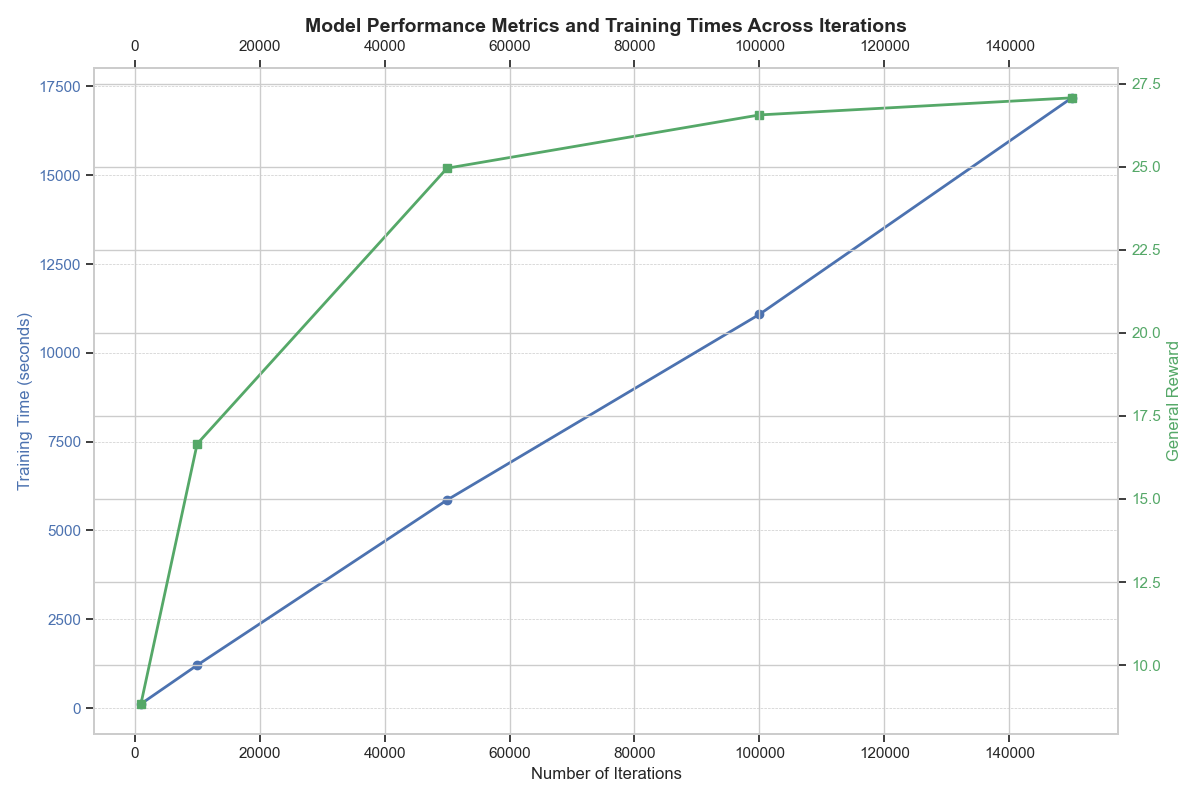
\includegraphics[width=\textwidth]{images/Iterations_plot_table.png}
    \caption{Performance metrics and training times for models trained with different step counts.}
    \label{fig:iterations_plot}
\end{figure}

\begin{table}[ht]
    \centering
    \renewcommand{\arraystretch}{1.4}
    \setlength{\tabcolsep}{12pt}
    \begin{tabular}{cccc}
    \hline
    \textbf{Steps} & \textbf{Avg Episode Duration (s)} & \textbf{Collision Rate (\%)} & \textbf{Training Time (s)} \\ \hline
    1,000    & 0.395 & 99.00 & 116    \\ \hline
    10,000   & 0.729 & 80.00 & 1,207  \\ \hline
    50,000   & 1.070 & 20.00 & 5,857  \\ \hline
    100,000  & 2.254 & 11.00 & 11,083 \\ \hline
    150,000  & 2.257 & 11.00 & 17,178 \\ \hline
    \end{tabular}
    \caption{Performance metrics after 1000 testing runs across models with various steps count.}
    \label{tab:performance_metrics}
\end{table}

Gathering results while performing Step 4 of this experiment, the data represented in Figure~\ref{fig:iterations_plot} and Table~\ref{tab:performance_metrics} was obtained. Training time, as expected, follows the proportional rise. An increase of step count by 1.5 from value 100000 to 150000, results in the training time being 1.55 times longer from 11083s to 17178s respectively, which satisfies proportionality manner under reasonable uncertainty due to the inconsistency of a computational unit. 

Observing the collision rate, it does not show the behaviour of any simple function, however, its general actions can be described as an unevenly decaying function. While the steps count grows tenfold from thousand to ten thousand, the collision rate goes slightly down by 19 per cent, whereas a latter fivefold jump triggers a rapid fall of the dependent variable by 60\%. 

The last two measurements do not show the gradual change of collision rate, meaning the most important drop of this value is to be observed on the steps ranging from 10 to 50 thousand. Regarding average time and general reward values, they show a similar dependency on step number, the considerable rise of results up to 50000 for general reward and up to 100000 for average episode time. Afterwards, both values tend to slow down the growth significantly. 

Considering all captured performance measures, the step count of 100000 appears optimal. It is a checkpoint of gradual performance improvements of the model, while higher values have a much weaker impact.

\subsubsection{Model Type 2 "\texttt{Highway-Merge Model}"}

The second model is used for performance comparison between TL models. The goal of training this model was to assess the effectiveness of the criticality method application. The learning process of this model implied principles of TL.

Firstly, the \emph{Merge-Env} environment was initialized, as the further training procedure would be conducted there. Afterwards, the pre-trained \texttt{Pure Highway Model} was loaded using the \texttt{model.load()} function. In a standard DQN initialization, random values are assigned to all weights inside the DQN. However, this time, the model was not initialized from scratch, but the weight values from \texttt{Pure Highway Model} were used as input to the training process of the DQN algorithm. Non-random values represent the knowledge base of the input model, which was acquired from the \emph{Highway-Env}.

Further, the model was trained in the \emph{Merge-Env} with 10000 steps. The purpose of this was to feed the experience of the merge environment into a model that already possessed a certain performance level in highway scenarios. This realized the simplest TL method, and thus the model will be later assessed together with the model obtained using the criticality approach.

\subsubsection{Model Type 3 "\texttt{Highway-Merge Criticals}"}

The third model type is the key algorithm to be explored in this thesis — the Criticality TL Model. This is the main experimental model to be further evaluated and assessed to determine if the criticality approach in TL is an effective strategy to be applied. The latter part will describe the steps by which this model was obtained:

Implementation of training has one major difference, in comparison to Model Type 2, the manual population of the Replay Buffer with critical states. All steps before the training part are identical to the model described above, whereas there is an additional step to be performed afterwards. Before the learning process is started, we need to fill the Replay Buffer with the critical states that were found, to ensure that exceptionally this set of states will be used throughout the training process. 

From the criticality analysis procedure described in Section ~\ref{sec:criticality}, there was a set of observations of states found, which corresponded to global and local peak values of criticality measurement. For the Replay Buffer, it is required to have not only a starting observation of a state, but also an action to be performed based on this observation, the reward received when the action is performed, the consequent observation obtained and the boolean value if the state, following critical, contains collision of the agent vehicle, or not. To determine the action, next observation, reward and collision the loaded pre-trained highway model was used. When inputting the critical observation into the model, it performs a decision-making step, based on the learned Q-Net. 

Following the described procedure, the model was obtained by applying TL based on an isolated set of critical states to the pre-trained highway model. The next step is to assess the performance quality of the resultant model and prove that the received results are stable and reproducible.

\subsubsection{Model Type 4 "\texttt{Pure Merge Model}"}

Compared with the fourth model, the general effectiveness of the TL applied in Model Types 2 and 3 can be evaluated. This model is trained similarly to highway model number 1, going through 100000 steps in a single environment, however instead of \emph{Highway-Env}, the \emph{Merge-Env} was taken. The purpose of training the corresponding model is to have reference measurements of the non-TL model to identify the level achieved by the Model of Type 3.

The training algorithm was borrowed from the one used in \texttt{Pure Highway Model}(described in Section~\ref{sec:dqn}), with a minor change: the \emph{Merge-Env} environment was applied. The value for steps count was also chosen to be 100000, taking results obtained in Section \ref{sec:model_highway} into account.

\subsection{Performance metrics}\label{sec:performance_metrics}

The key to performance assessment is the choice of metrics to be collected during the evaluation of models. The right set of resultant data will enable a deeper analysis of performance. Moreover, the combination of various outputs can show unexpected dependencies and valuable trends. 

Three identical sets of 1000 episodes were offered to Model Types 2, 3 and 4 as an environment to perform a "test drive" and to measure the effectiveness of algorithms. Every model ran through 1000 episodes of merge environment, and the following data was captured and saved for later analysis:

\subsubsection{Rewards}\label{sec:rewards_types}

While driving, the \emph{Merge-Env} accesses the driving behaviour of the agent vehicle according to multiple criteria and, based on this, rewards the vehicle. Reward values are combined into a dictionary with keys set to reward categories and values being lists of reward points received. There are 6 categories to be accessed in the \emph{Merge-Env}:

\begin{itemize}
    \item \textbf{Collision reward} (\texttt{"collision\_reward"}) -- a penalty to be received by the vehicle in case of a collision. The purpose of the collision reward is to reduce points, encouraging an algorithm to prioritize safety by avoiding hazardous situations.
    \item \textbf{Right lane reward} (\texttt{"right\_lane\_reward"}) -- the reward is received when the agent is continuously driving in the far-right driving lane.
    \item \textbf{High-speed reward} (\texttt{"high\_speed\_reward"}) -- when the agent drives while maintaining a high speed, the high-speed reward is granted.
    \item \textbf{Merging speed reward} (\texttt{"merging\_speed\_reward"}) -- this is an altruistic reward granted to the ego vehicle depending on the velocities of all vehicles except for the merging vehicle. The formula is~\cite{highway-env}:
    \begin{equation}
 R_{\text{merge}} = \sum_{i \in \mathcal{V}_{\text{merge}}} \frac{v_i^{\text{target}} - v_i}{v_i^{\text{target}}},
        \label{eq:merging_reward}
    \end{equation}
 Where \(\mathcal{V}_{\text{merge}}\) is all vehicles except for the one driving in the merging lane, \(v_i^{\text{target}}\) is set to 30 in the \emph{Merge-Env} implementation, and \(v_i\) is the velocity of the chosen vehicle. The reward is named altruistic because it examines the velocities of all vehicles, encouraging cooperative behaviour, where the agent synchronizes its speed with neighbouring traffic to ensure the smoothness of a merging scenario.
    \item \textbf{Lane change reward} (\texttt{"lane\_change\_reward"}) -- a reward to be granted when a lane change action is performed, either \texttt{LANE\_RIGHT} or \texttt{LANE\_LEFT} action.
    \item \textbf{General reward} (\texttt{"general\_reward"}) -- a combined value of all rewards and penalties received during one action step of the agent. The value is received as an output of the function \texttt{env.step(action)}. The value is summed throughout all action steps inside a single episode.
\end{itemize}

\subsubsection{Collisions}\label{sec:collisions}

The boolean value represents if the episode was terminated due to a collision. Keeping track of these metrics will help in identifying the collision rate of the ego vehicle. Calculations of the collision rate are performed with the use of the following formula:
\begin{equation}
 \text{Collision Rate} = \frac{N_{\text{collision}}}{N_{\text{total}}},
    \label{eq:collision_rate}
\end{equation}
where \(N_{\text{collision}}\) is the number of episodes which ended with a collision of agent vehicle, is divided by \(N_{\text{total}}\) total number of episodes(1000).

\subsubsection{Episode duration}\label{sec:duration}

The duration of an episode is the measure to collect information about the driving time of the agent. Throughout the implementation, episode duration is collected in the following way: at the beginning of an episode, the current timestamp is saved to a variable using \texttt{time.time()} function, later when the episode is finished, the starting time is subtracted from the current timestamp at the end of an episode, resulting into the episode duration.

\subsubsection{Criticality values}\label{sec:criticality_values}

Additionally, the array of criticality values(variance of Q-values) is collected during the examination of models. Sets are obtained via the algorithm described in Section ~\ref{sec:criticality} of this thesis. The purpose of this metric is to observe not only the performance of models but also the distribution of state criticality throughout episodes. The hypothesis is that the model trained with the Replay Buffer of critical states should have fewer states when the criticality value is high. This will be explored via the criticality distribution plot further.

\subsection{Reproducibility test}\label{sec:reproducibility_test}

Approaching the measurement of the reliability of the criticality method, along with its performance, it was decided to conduct 10 experiments. The number of tests was taken to be 10 due to the duration of every experiment. All in all, each experiment consists of multiple steps, with the final point being to train the model based on the critical observations. The steps preceding the last one were performed to prepare the criticality data for the target model; and obtain models that will be included in the final assessment procedure of the experimental algorithm. As for the steps of a single experiment:

\begin{enumerate}
    \item Train the model, based purely on \emph{Highway-Env} with the steps count equal to 100000. This model was obtained following steps explained in Section ~\ref{sec:dqn} of this thesis;
    \item Apply the TL to the pre-trained \emph{Highway-Env} model. The initial model from Step 1 is fed with 10000 steps of \emph{Merge-Env} to gain experience of a new environment with additional complexity in the face of merging lanes and vehicles. The TL process used during this step will later be upgraded by isolating the training data sampling process to only critical states;
    \item Test the model obtained in Step 2 through 1000 episodes of \emph{Merge-Env}, collecting the metrics listed in Section ~\ref{sec:performance_metrics}. Gathered performance data will further be used in comparison purposes while estimating the resultant effectiveness of \texttt{Highway-Merge Criticals} model;
    \item Prepare the set of critical state observations by running the Step 1 \emph{Highway-Env} model for 1000 episodes of \emph{Merge-Env}. The collected testing data is similar for every evaluation process;
    \item Train the experimental TL model based on the adjusted Replay Buffer. The used Experience Replay Buffer was populated purely with critical state observations gathered in Step 4, and additional information about the action, reward, and following state observations, was obtained via the decision-making process of the \emph{Highway-Env} model from Step 1. The result of this step is the goal model of this paper;
    \item Rate the \texttt{Highway-Merge Criticals} model through 1000 episodes of \emph{Merge-Env}, saving all obtained results;
    \item Train a reference \emph{Merge-Env} model without applying TL—going through 100000 steps learning process inside \emph{Merge-Env};
    \item Compile the assessment results for the reference model in Step 7 with the evaluating process analogous to the ones described in Steps 3, 4, and 6.
\end{enumerate}

After all necessary measurements for every obtained model are gathered and saved, it is time to visualise the data and, based on this, draw conclusions. There are various ways to represent the data in a clear and accessible way, but I tried to find the most crucial formats and describe them further. 

\subsection{Discussion of results}

This part focuses on explaining results gathered throughout conducted experiments and discussing observations and conclusions to be derived from visualised results.

\subsubsection{Number of critical observations}\label{sec:n_critical_observations}

Each of the 10 experiments had a different seed number to control obtained models. The randomness value was kept fixed throughout the experiment and applied only while training. However, the evaluation of all models was conducted on the set of 1000 environment states where seed numbers were spread between numbers 2000 and 2999. The seed number enables the reproducibility of experiments and creates different starting conditions while performing every test. Due to the variability of initial conditions during training of \emph{Highway-Env} model, a different number of critical observations was produced by Step 4 of the algorithm, described in Section ~\ref{sec:reproducibility_test}. 

\begin{figure}[H]
    \centering
    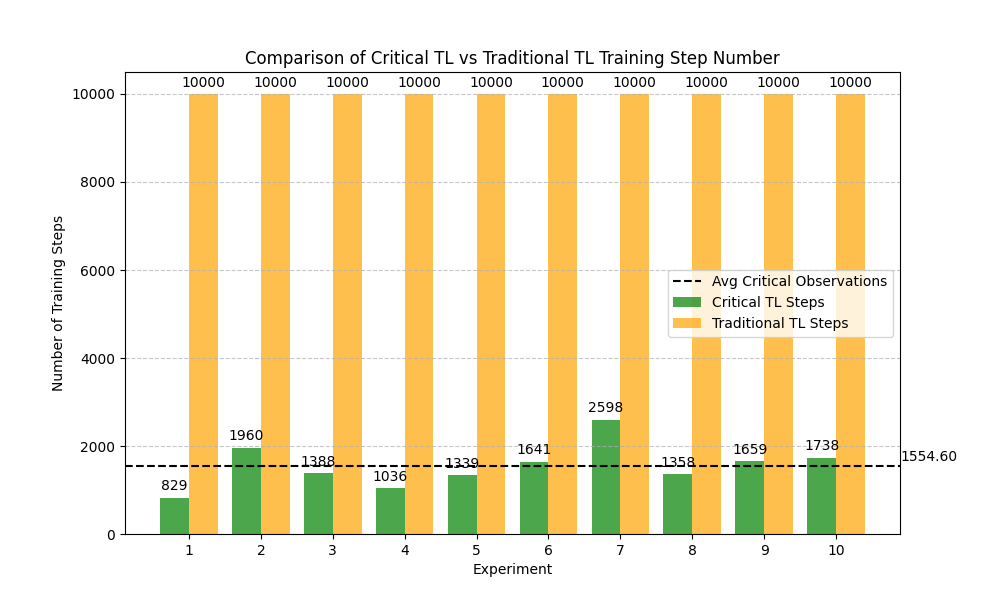
\includegraphics[width=\textwidth]{images/Crit_obs_count.png}
    \caption{The distribution of the number of critical states collected and used for training in each experiment}
    \label{fig:crit_obs_count}
\end{figure}

Figure \ref{fig:crit_obs_count} visualises the training steps count for two TL models during each experiment. Moreover, blue bars represent the number of critical states(identification method is explained in Section \ref{sec:criticality}) that were fed into the Replay Buffer(Step 5 in Section ~\ref{sec:reproducibility_test}) while training the \texttt{Highway-Merge Criticals} model in every test step. It can be seen that by changing the seed number a variety of training data for the target model was produced. This made it possible to search for interconnections between the number of critical states and the performance of the obtained model.

As the step number for traditional TL was fixed to 10000 and the number of critical states found differs from test to test, the time gain is also variable. However, taking the mean value of critical states, the training of TL with a criticality approach was 6.4 times faster than that of the traditional TL algorithm.

However, the comparison of the models' training time was not fully accurate. This limitation arises from the fixed number of training steps for traditional TL. There the optimal performance could have been achieved in fewer steps. Due to that, the time reduction between the two TL approaches cannot be accessed objectively. The examination of learning curves of trained models can be helpful in analysing the training time of different methods. By evaluation of the model evolving throughout the training, deeper insights can be achieved.

\subsubsection{Collision rate}\label{sec:collision_rate}

When addressing the performance and reliability of dynamic environments, such as autonomous driving, models the collision rate tends to be a crucial metric. Given the proportion of episodes where collisions occur, it provides a fair measure of safety. Through the analysis of collision rates across various model types and different experiment conditions, different insights into model behaviour can be revealed. For instance, the effectiveness of TL, or the effect of the application of critical states on the decision-making process.

\begin{figure}[H]
    \centering
    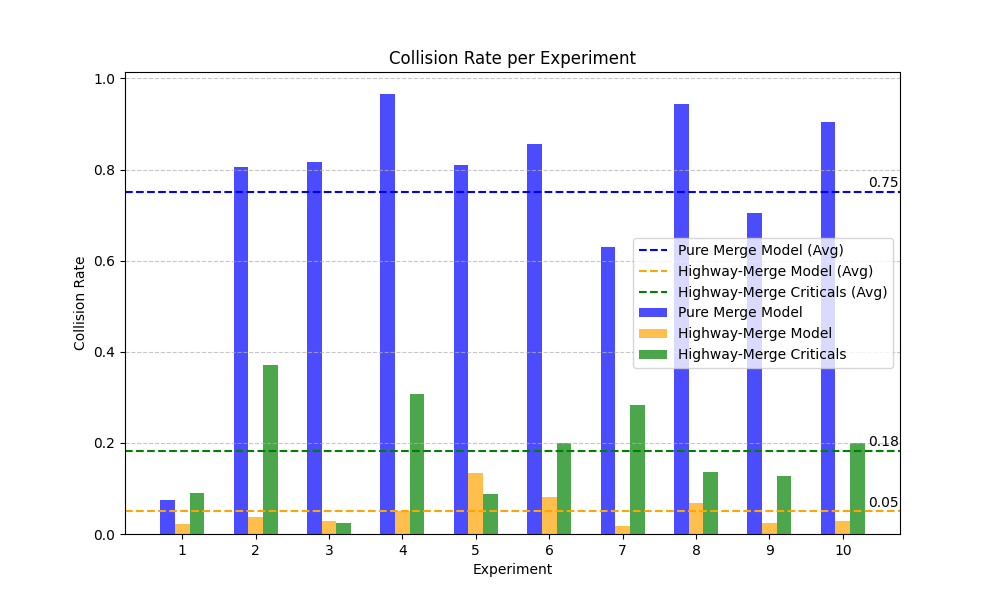
\includegraphics[width=\textwidth]{images/Collision_rate.png}
    \caption{Agent's collision rate per experiment for each model.}
    \label{fig:collision_rate_plot}
\end{figure}

Throughout 10 experiments, the collision boolean value was tracked. It takes a True value if the episode finished due to an accident, and a False value otherwise. Taking into account booleans from all 1000 episodes of each experiment, the plot in Figure \ref{fig:collision_rate_plot} was created. A single point on a graph represents a collision rate value, calculated using a formula described in Section ~\ref{sec:collisions}. The x-axis of a plot defines the experiment step number and the y-axis represents collision rate values, which occupy a continuous interval from 0.0 to 1.0.

In Figure \ref{fig:collision_rate_plot}, there are relatively low collision rate values to be observed for all models, including some fluctuations around the average value and outliers. In general, the concentration of values is to be found between 0.0 and 0.35, as for average values, an even smaller range is to be occupied. 

\texttt{Pure Merge Model} model shows not only the most unstable behaviour among all but also has an extremely high level of unsafety. Owning an average collision rate of 0.75, it shows the worst performance. On average approximately 750 episodes out of a total number of 1000 ended up with the crash. Moreover, among all tests, there were 3 where the accident rate rose to the level of 95\%, meaning that in almost 1/3 of conducted experiments, the probability of a car finishing the episode safe was only 5\%. If, theoretically, this model was implemented inside of a real autonomous vehicle, it would have been extremely dangerous to use following cars.

Despite generally terrible performance metrics, there is an outlier to be noticed in the graph of \texttt{Pure Merge Model}. In the first evaluation task, the model shows a collision rate of only 0.1 as an average value of 1000 runs. Such a huge drop is to be explored further with other plots.

Generalising the behaviour of a pure   RL algorithm, the higher average collision rate of the model, if compared to others, reflects its limitations while being trained solely on the \emph{Merge-Env}. It lacks the variability of experience and abilities to deal with complex merging scenarios, making it highly prone to collisions. 

The lowest average collision rate of 0.05 is achieved by the \texttt{Highway-Merge Model}. Based only on the collision rate, its performance is stable and safe. Comparing the number of input states, used while performing TL, it can be seen how 10000 random states, used for this model, outperform the lower number of total states used in \texttt{Highway-Merge Criticals}. The orange graph remains stable in the scope of most test drives, although having two moderate peaks during experiments 5 and 7. Nevertheless, the rise of jumps concerning an overall average of 0.05, is only 0.1 and 0.03 respectively.

Focusing on the \texttt{Highway-Merge Criticals} model, it shows middle values among other trendlines. Compared with \texttt{Highway-Merge Model}, it has bigger deviations from the mean value, behaving astatically. During experiments 3 and 5, it achieved a collision rate lower than \texttt{Highway-Merge Model}, while experiments number 4, 8 and 10 had more collisions than others. There can be 3 peaks of collision rate observed in the 2nd, 4th and 7th tests, which indicates a lower safety level of driving as approximately every 3rd driving episode ended with an accident. Referring to the Figure \ref{fig:crit_obs_count} data, the mean number of collected critical states can be calculated, it is 1554.6. While utilising, on average, a 6.4 times smaller set of TL input states, \texttt{Highway-Merge Criticals} model has a mean collision rate of only 3.6 times higher than the one of \texttt{Highway-Merge Model}. This comparison indicates potential improvements that can be achieved through the use of the criticality method within the scope of TL.

\subsubsection{Average episode duration}\label{sec:episode_time}

An additional metric that represents the reliability of the autonomous driving agent is the average time of an episode. The duration of an episode has a direct connection to the safety of an algorithm.

Observing Figure~\ref{fig:avg_times_plot} and taking into account the values range of the average episode time, it is worth saying that the time measure is relative. The number of seconds to be captured from the beginning to the end of the episode takes values of within 1 second due to the rendering speed of the \emph{Highway-Env} environment, this time cannot be referenced as a real-time measure. 

Analysis of the general behaviour of three trendlines, presented in Figure~\ref{fig:avg_times_plot}, shows the pure superiority of the TL approach over the basic RL, applied in the \texttt{Pure Merge Model}. Here, average values for TL models differ only by 0.03 seconds, whereas the third model owns a mean episode duration value of 0.52s after 10 experiments. \texttt{Pure Merge Model} shows an incredible performance instability with the interval of values of 0.85 seconds and 0.35 seconds. 

The first test drive is to be considered exceptional. This is because the data gathered for experiment 1 does not follow general trendlines in either of the three metrics that have already been explored. This test shows an overall average episode time taking the highest values among all experiments for all three models, without exceptions. Additionally, the accident rate for every model is relatively low, especially the \texttt{Pure Merge Model} value demanding attention. The collision rate of an unbelievable 10\% is a suspiciously tiny number if compared with a standard range of values from 65\% at the lowest point and 95\% at the highest. Notwithstanding, the critical observations count is the smallest among 10 experiments, only of 829 samples. Thus episode 1 is to be excluded from the further discussion of general metrics' behavior.
\begin{figure}[H]
    \centering
    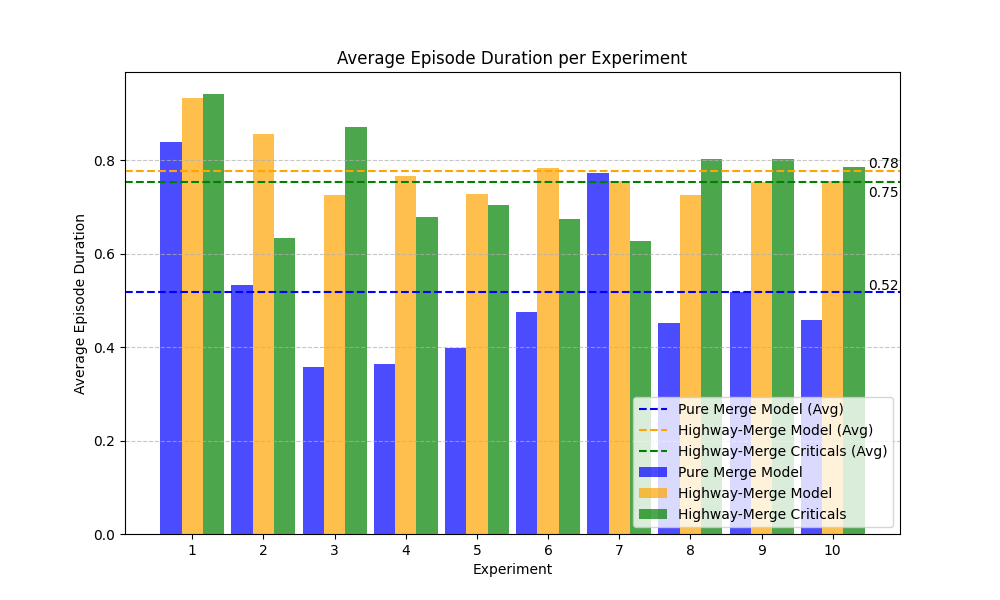
\includegraphics[width=\textwidth]{images/Average_times_plot.png}
    \caption{The plot of an average episode duration per experiment for every model.}
    \label{fig:avg_times_plot}
\end{figure}

Through analysis of the abnormal behaviour of a model \texttt{Pure Merge Model} within the first experiment, one theory was proposed. The following results could only be obtained if the set of randomized initial conditions for the experiment was created in such a way that the model was able to perform much better decision-making, and thus result in a higher value of episode time and a lower collision rate. Based on those two metrics the resultant number of critical observations was reasonably smaller.

The best result of a blue graph(if not taking episode 1 into account) was reached during episode number 7. Taking the data from Figures \ref{fig:crit_obs_count} and  \ref{fig:collision_rate_plot} into account, in the 7th episode \texttt{Pure Merge Model} shows a local peak value of average experiment time of 0.77 seconds while having the best collision rate and collecting the most number of critical observations of 2598. 

There is a strong logical and quantitative correlation between those 3 metrics to be explored via the 7th task. As the agent was able to avoid accidents in approximately 37\% of episodes, the mean runtime value increased up to 0.77s. The combination of longer episode time and lower collision rate boosted the number of critical states that were found during this run. The increase of critical states number from a medium value of approximately 1500 observations rocketed up to almost 2600 observations, which is a total of 173,3\% from a mean value. Similar behaviour is also visible in episodes 2 and 9, albeit on a smaller scale.

As of \texttt{Highway-Merge Model}, average episode times follow a similar pattern if compared to the collision rate graph. It remains relatively stable around an average value of 0.78, with some fluctuations occurring in a range of 0.05 seconds more or less.

Exploring results of experiments where \texttt{Highway-Merge Criticals} was controlling the agent vehicle interesting observations were found. Even though the average value is not of big different from the second TL model, the graph is not as smooth as in the other model. There is one global peak to be seen in experiment 3 and two experiments where the value hit the lowest point(experiments number 2 and 7). Both dips of a graph in tests 2 and 7 are accompanied by peaks of a collision rate. Whereas, during the peak value of 0.97s run in experiment 3, the accident rate value drops to the lowest point of the graph of only 3\%, which corresponds to the generalised interconnection of those metrics described above.

Based on the driven conclusion to exclude episode number 1 from the overall statistics, new average values were calculated(analogically to dashed lines, denoted on Figures \ref{fig:avg_times_plot} and  \ref{fig:collision_rate_plot}). The Table~\ref{tab:overall_averages} defines newly calculated values:

\begin{table}[ht]
    \centering
    \renewcommand{\arraystretch}{1.4}
    \setlength{\tabcolsep}{12pt}
    \caption{Overall Averages for every model (Excluding Experiment 1)}
    \begin{tabular}{lcc}
    \hline
    \textbf{Model} & \textbf{Avg Collision Rate} & \textbf{Avg Episode Time} \\ \hline
 Merge 100000 steps & 0.8264 & 0.48 \\ \hline
 Highway-Merge Model     & 0.0524 & 0.76 \\ \hline
 Highway-Merge Criticals & 0.1931 & 0.73 \\ \hline
    \end{tabular}
    \label{tab:overall_averages}
\end{table}

Average values for accident rates of models which employed TL, if excluding the first experiment, changed by a mean of 5\%, whereas for \texttt{Pure Merge Model} this value rose by 10\% up to 0.83. Analysing the consequences of the experiment number diminishing for the average episode time graph, the following results appeared: all values went down, however, the variation of the pure RL model was twice as big as other models, and time dropped down by 0.04s, with others only experiencing a decline of 0.02 seconds. In total, the statistics have not changed much, when removing the outlier.

\subsubsection{General rewards}\label{sec:gen_rewards_results}

\begin{figure}[H]
    \centering
    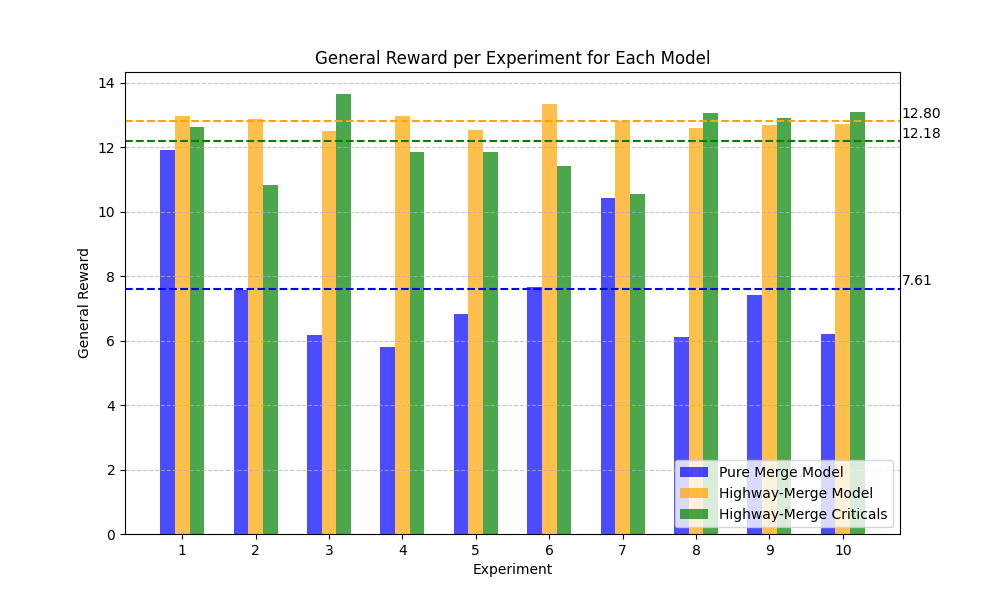
\includegraphics[width=\textwidth]{images/General_rewards.png}
    \caption{The plot of an average general reward per experiment for every model.}
    \label{fig:gen_rewards}
\end{figure}

The system of rewards is a crucial component of RL's idea. In unsupervised learning, in complex and dynamic environments where the set of all possible outcomes is not possible to simulate and even more so to calculate the most optimal route in advance, the Q-learning strategy is to be applied. There, Q-values are calculated with the use of possible prospective reward to be received by the agent if a particular action was taken, as written in Equation~\ref{eq:q_value}.

Figure~\ref{fig:gen_rewards} represents one of the multiple types of collected rewards (as described in Section~\ref{sec:rewards_types}) the general reward. If comparing Figures \ref{fig:avg_times_plot} and \ref{fig:gen_rewards}, a striking resemblance of those graphs can be seen. The behaviour of graph lines for every model shows similar patterns with small deviations and scaling differences. As explained above, the reward value has a direct influence on the actions taken throughout the decision-making process, and thus on the results of time measurements for 1000 episodes of every test. Peaking values of average time correspond to the peaking result of a general reward, and vice versa.

\subsubsection{Overall Rewards Comparison by Reward Types}\label{sec:overall_reward_types}

For statistics purposes and as a chance to understand the behaviour of different types of models there were data about all possible types of rewards collected. Measurements of all 6 types of received rewards, described in Section \ref{sec:rewards_types}, were separately connected. Figure~\ref{fig:rewards_all} represents average values of rewards among 10 experiments by model and reward type.

\begin{figure}[H]
    \centering
    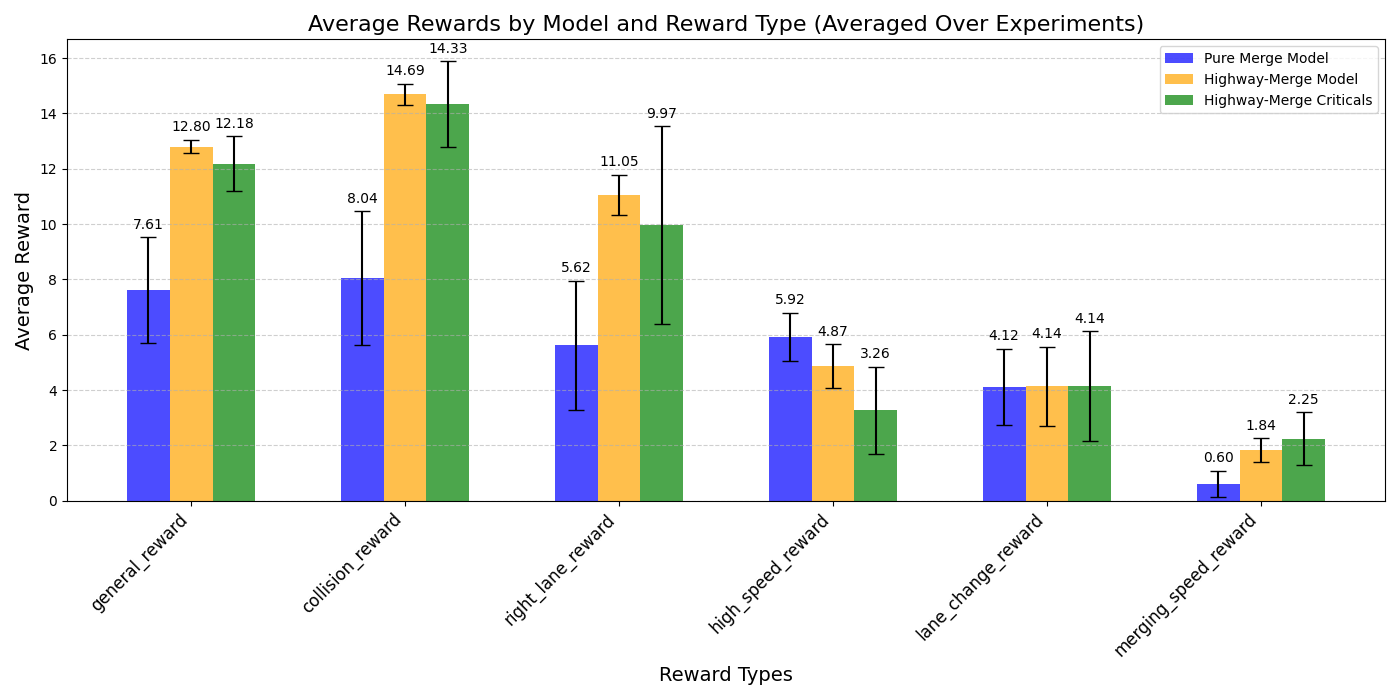
\includegraphics[width=\textwidth]{images/Rewards.png}
    \caption{Error bar plot of rewards, averaged over 10 experiments, by model and reward type.}
    \label{fig:rewards_all}
\end{figure}

The general reward value was already explored deeper in Section~\ref{sec:gen_rewards_results}, however, this reward type defines only the total performance of the model. Whereas other types help find out what is the direction of decision-making that was applied throughout the tests.

Analysis of the collision reward should be conducted relying on the collision rate graph, too. If compared with the collision rate, collision reward gives reasonable results. The highest average collision reward is owned by the \texttt{Highway-Merge Model}, due to the lowest mean value of a collision rate depicted on Figure~\ref{fig:collision_rate_plot} of only 0.05. The second highest value of collision reward, with a difference of only 0.34, has \texttt{Highway-Merge Criticals} model. This matches with the data obtained for the accident rate, where TL models showed better performance than the \texttt{Pure Merge Model}. The reward value obtained by \texttt{Pure Merge Model} due to accidents managing abilities of a model is almost twice as low as ones of other models. A similar tendency is also plotted on the collision rate graph, which demonstrates the inability of the pure RL model to drive safely, omitting collisions.

Going further to the right lane reward does not change the overall situation entirely, the ranking of models remains unchanged. The blue bar has the worst result of 5.62, showing that this model was prone to take the middle of the leftmost lane during the episode. At the same time, the other two models perform a lot better at right-lane keeping throughout experiments. For better performance, the results of 9.97 and 11.05 were granted to models \texttt{Highway-Merge Criticals} and \texttt{Highway-Merge Model} respectively. 

Points, with which the model is rewarded when driving with a high speed, show an exceptional distribution among models. The first and the only time \texttt{Pure Merge Model} showing the best result among all. 5.92 is the high-speed reward owned by this model, whereas other models received a lower reward by driving slower. 

Direct connection between collision and higher speed can be observed if taking into account the lane change reward. Showing almost identical values for this reward, with a small difference of only 0.02, models decided to change the lane on average an equal number of times. As a lane change reward is received if lane change action was taken(additionally described in Section~\ref{sec:rewards_types}), it does not consider the success of this action, thus this can be observed by observing collision and high-speed rewards. Among an equal number of lane change attempts, considering driving with the highest speed of all models, \texttt{Pure Merge Model} succeeded almost twice as rare as others. This means that a trained policy of \texttt{Pure Merge Model} prioritised driving faster than avoiding collisions with surrounding vehicles. If digging into the policy of \texttt{Highway-Merge Criticals} model, it can be seen, that being trained on a smaller set of critical states than \texttt{Highway-Merge Model}, it learned to retain a lower speed to avoid accidents effectively. By following this strategy it almost succeeded in receiving a collision reward as high as one of the second models. 

The last reward metric to be explored is the one for merging speed(the formula used to calculate the value of this reward is described in Section~\ref{sec:rewards_types}). The best value for this reward was achieved by \texttt{Highway-Merge Criticals} model, indicating the best cooperative behaviour of agent vehicles among all. Second and third places are taken by \texttt{Highway-Merge Model} and \texttt{Pure Merge Model} respectively. 

If looking at the standard deviation of values, the following observations can be seen. Throughout almost all values the upper boundary of the confidence level of \texttt{Highway-Merge Criticals}, the average value plus standard deviation of the value, reaching higher values than ones of \texttt{Highway-Merge Model}. This behaviour can be seen for all metrics except for high-speed reward. The higher overall standard deviation of rewards of \texttt{Highway-Merge Criticals} defines the lower stability of this model. For instance, the deviation of results for a general reward of the research model is noticeably higher than ones of \texttt{Highway-Merge Model}; this shows that despite that on average the reward is lower, the performance of the critical model is better in some experiments, which can be observed on Figure \ref{fig:gen_rewards}. Similar behaviour can be observed with collision reward when looking at values of this metric through single experiments on Figure \ref{fig:collision_rate_plot}.